% Copyright (c) 2016 Laboratory for Bionic Communication Engineering
% Released under the MIT license

\documentclass[a4j, twocolumn, openleft, uplatex, dvipdfmx]{jsbook}

\usepackage{newtxtext}
\usepackage{graphicx}
\usepackage[uplatex, deluxe]{otf}
\usepackage{tikz}
\usepackage{here}
\usepackage{hyperref}
\usepackage{pxjahyper}
\usepackage{pdfpages}

\usetikzlibrary{positioning}

\title{\textgt{生体アンプの使い方}}
\author{\textgt{生体通信工学研究室}}
\date{}

\begin{document}
    \maketitle

    \tableofcontents

    \chapter{準備}
    \label{chap:準備}

    \section{準備するもの}
    \label{sec:準備するもの}

        \subsection*{生体アンプ}
            \begin{figure}[H]
                \centering
                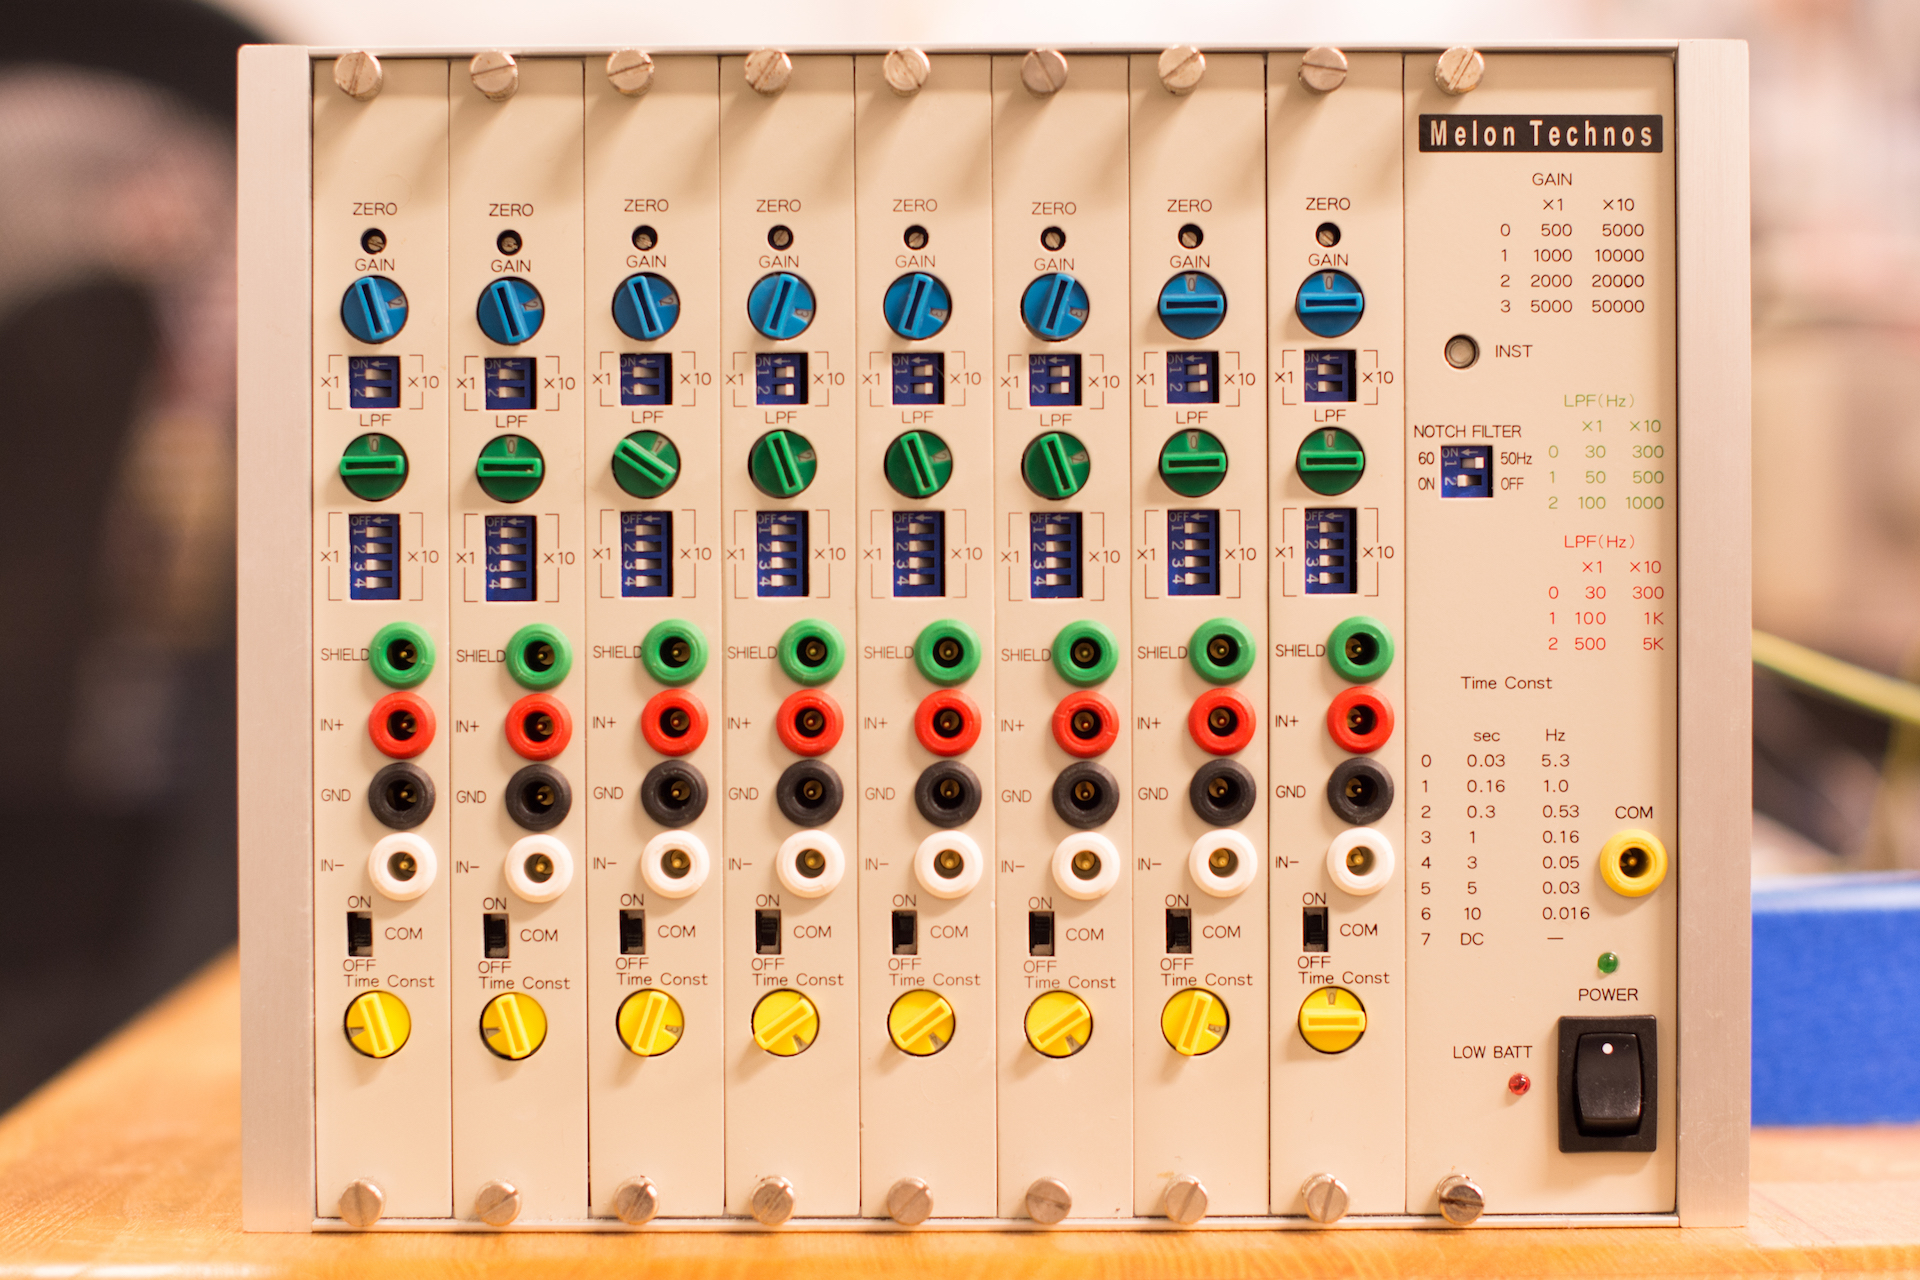
\includegraphics[width=0.6\linewidth]{./figure/amp.jpg}
            \end{figure}
        \subsection*{生体アンプのバッテリ}
            \begin{figure}[H]
                \centering
                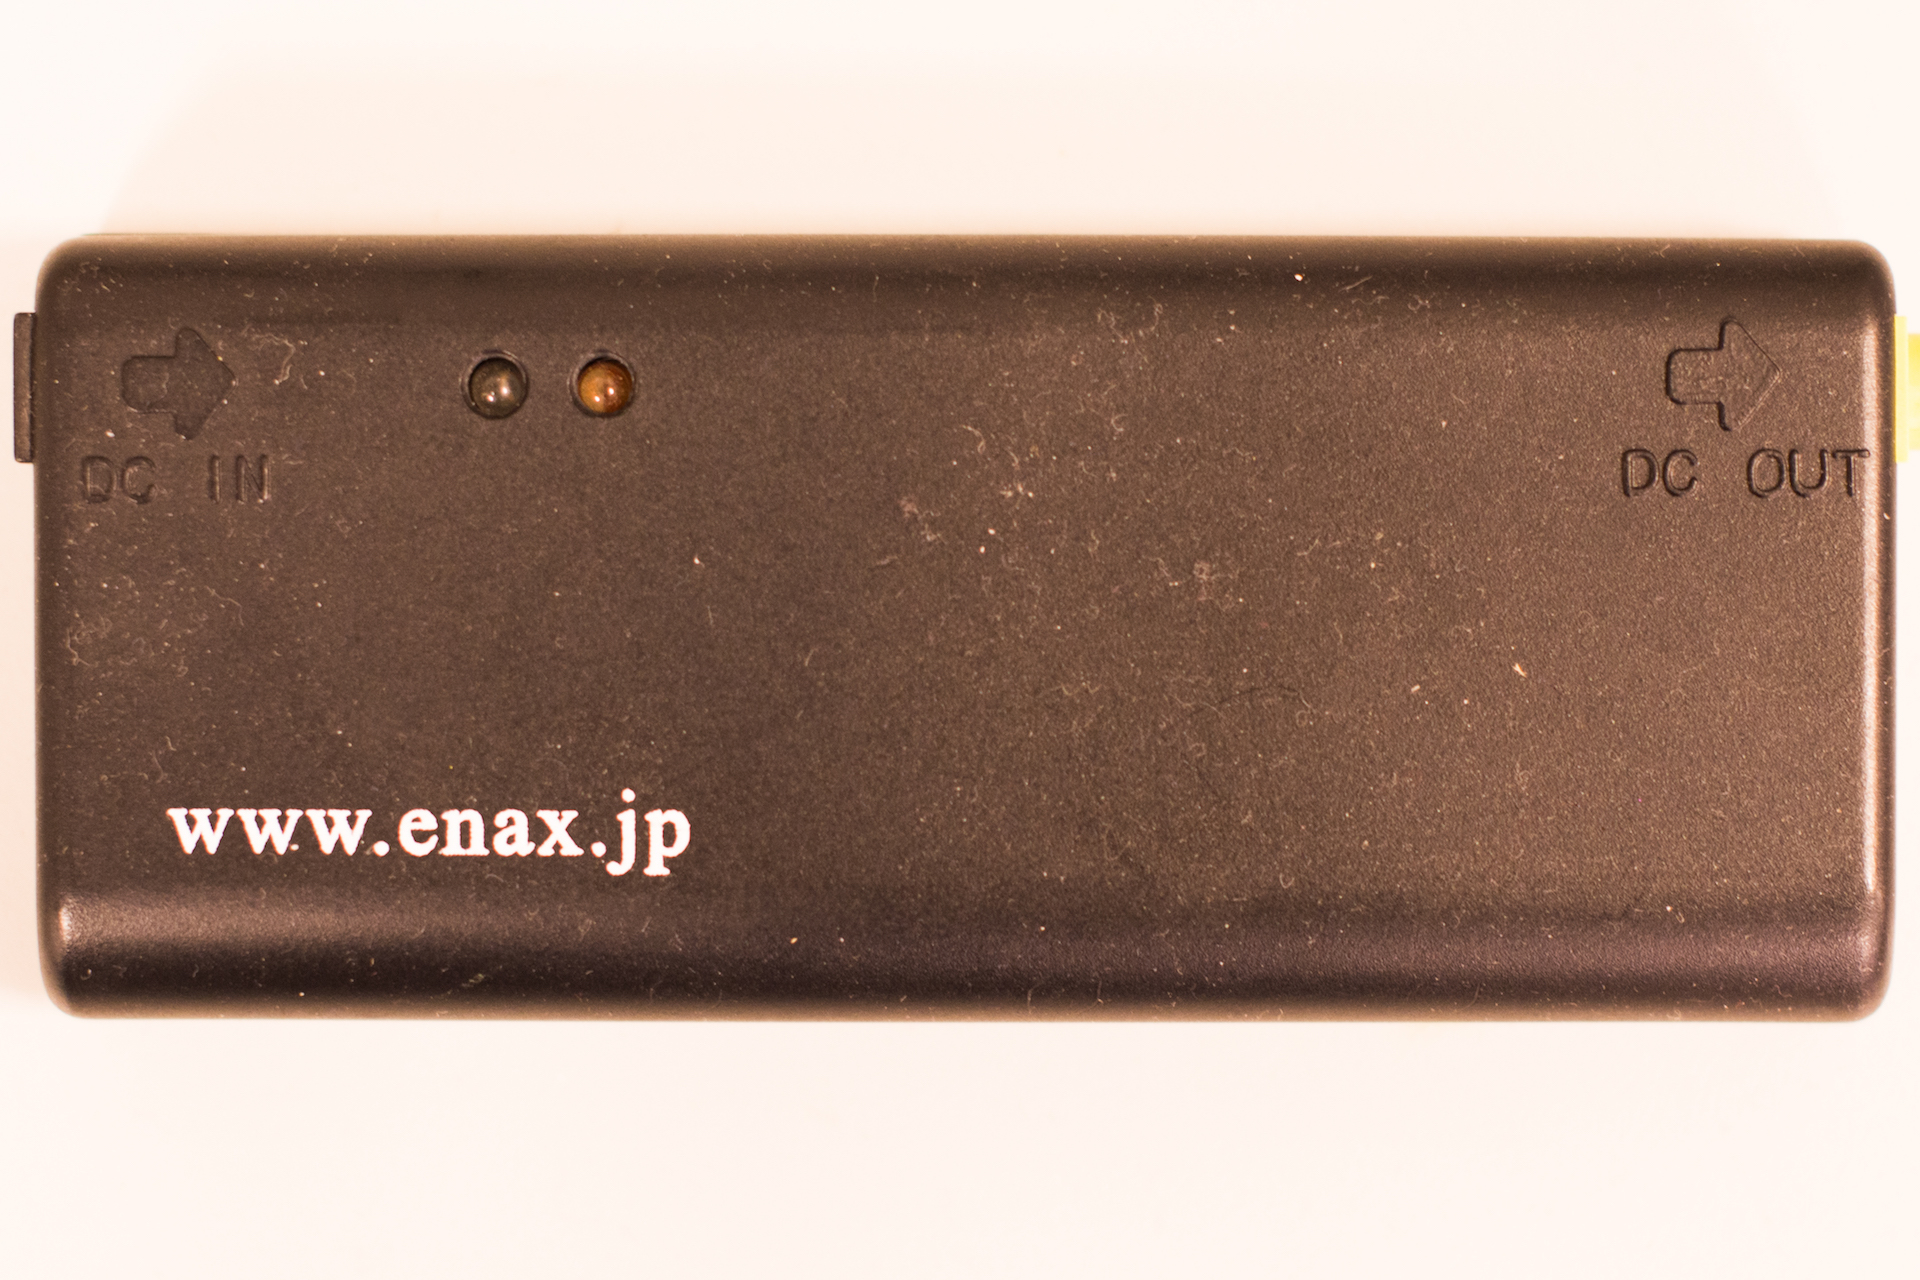
\includegraphics[width=0.6\linewidth]{./figure/battery.jpg}
            \end{figure}
        \subsection*{データレコーダ}
            \begin{figure}[H]
                \centering
                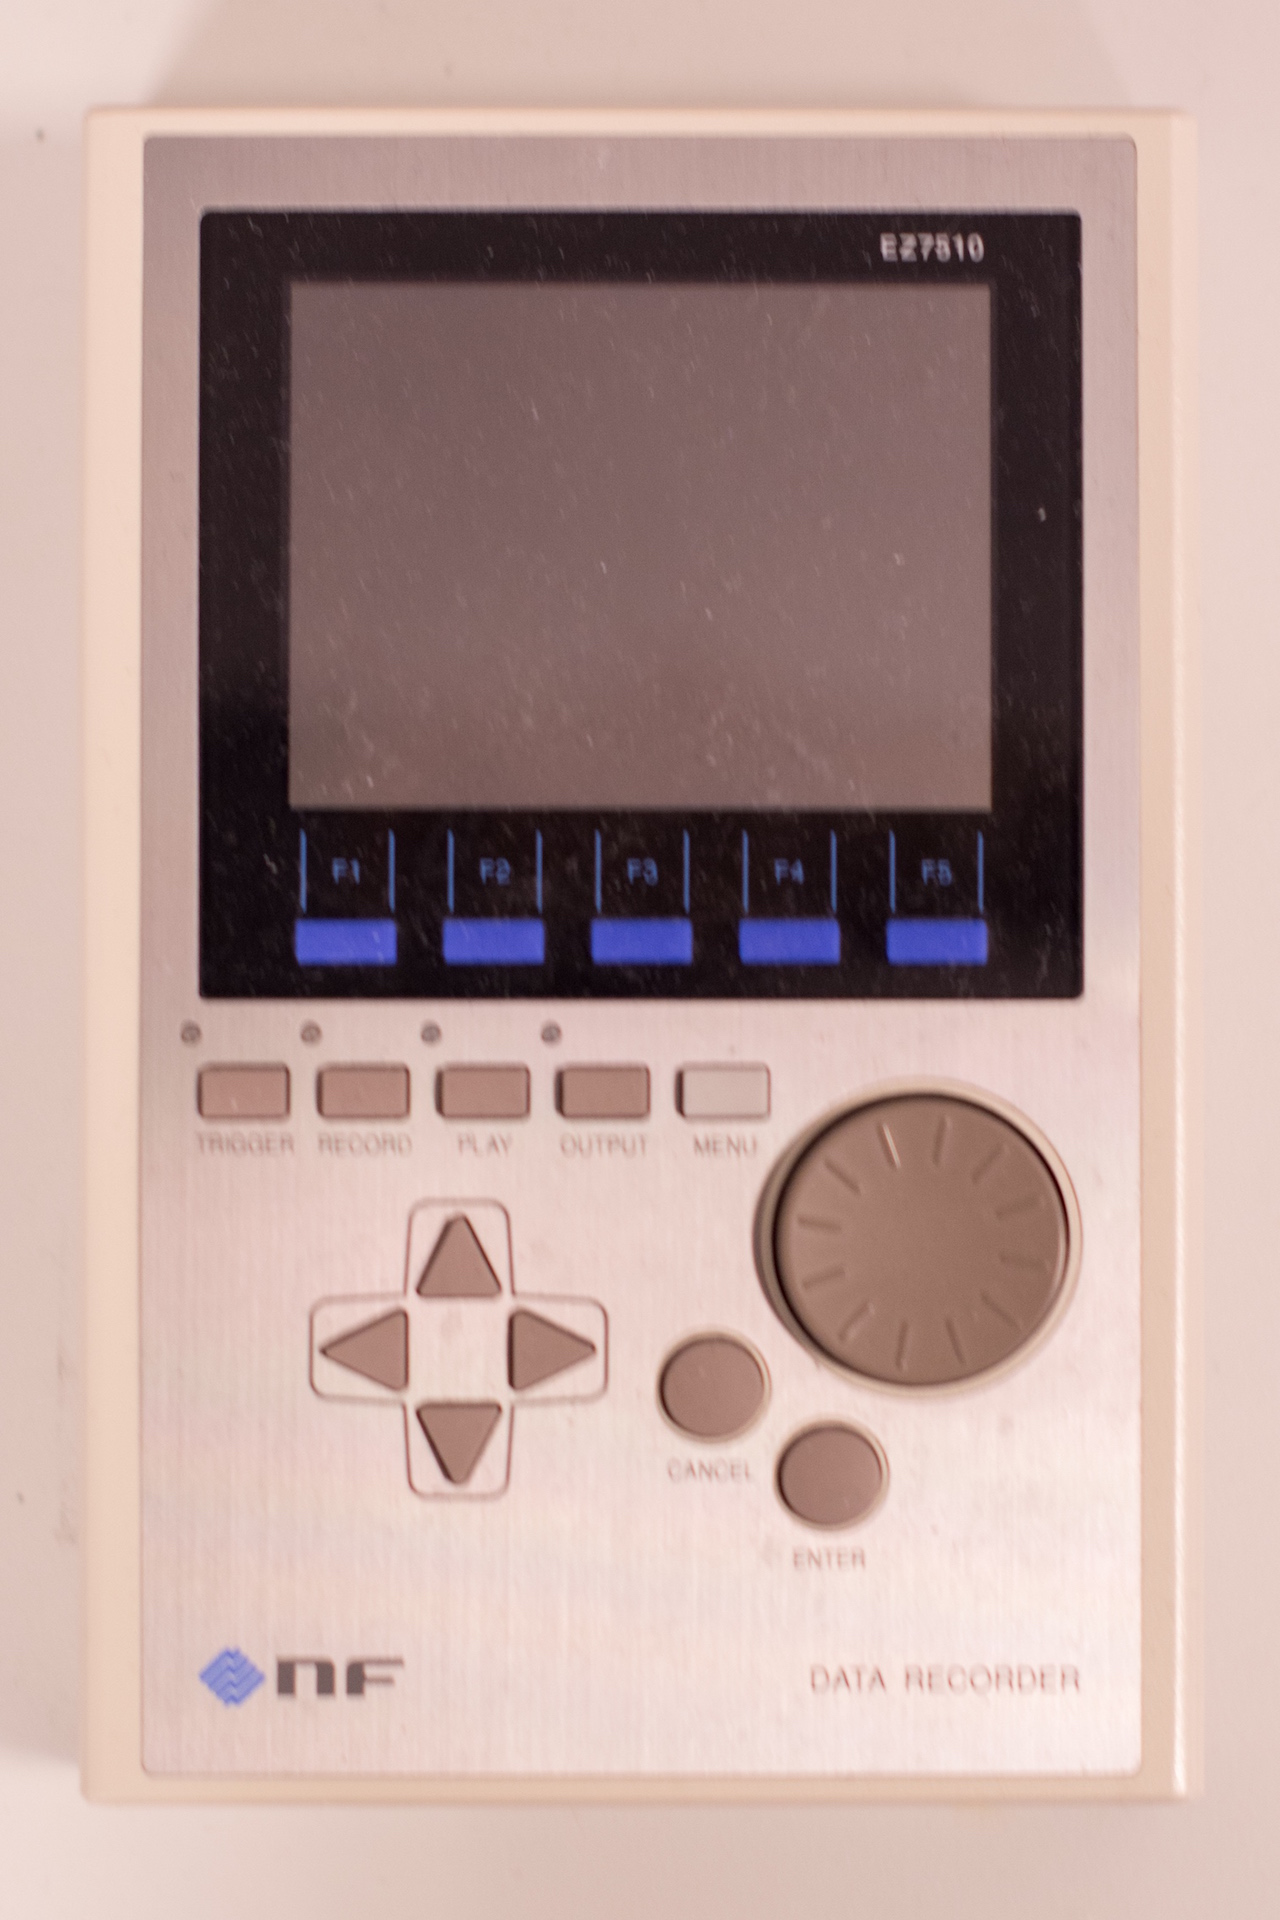
\includegraphics[width=0.5\linewidth]{./figure/nf.jpg}
            \end{figure}
            通称「ゲームボーイ」
        \subsection*{BNCボックス}
            \begin{figure}[H]
                \centering
                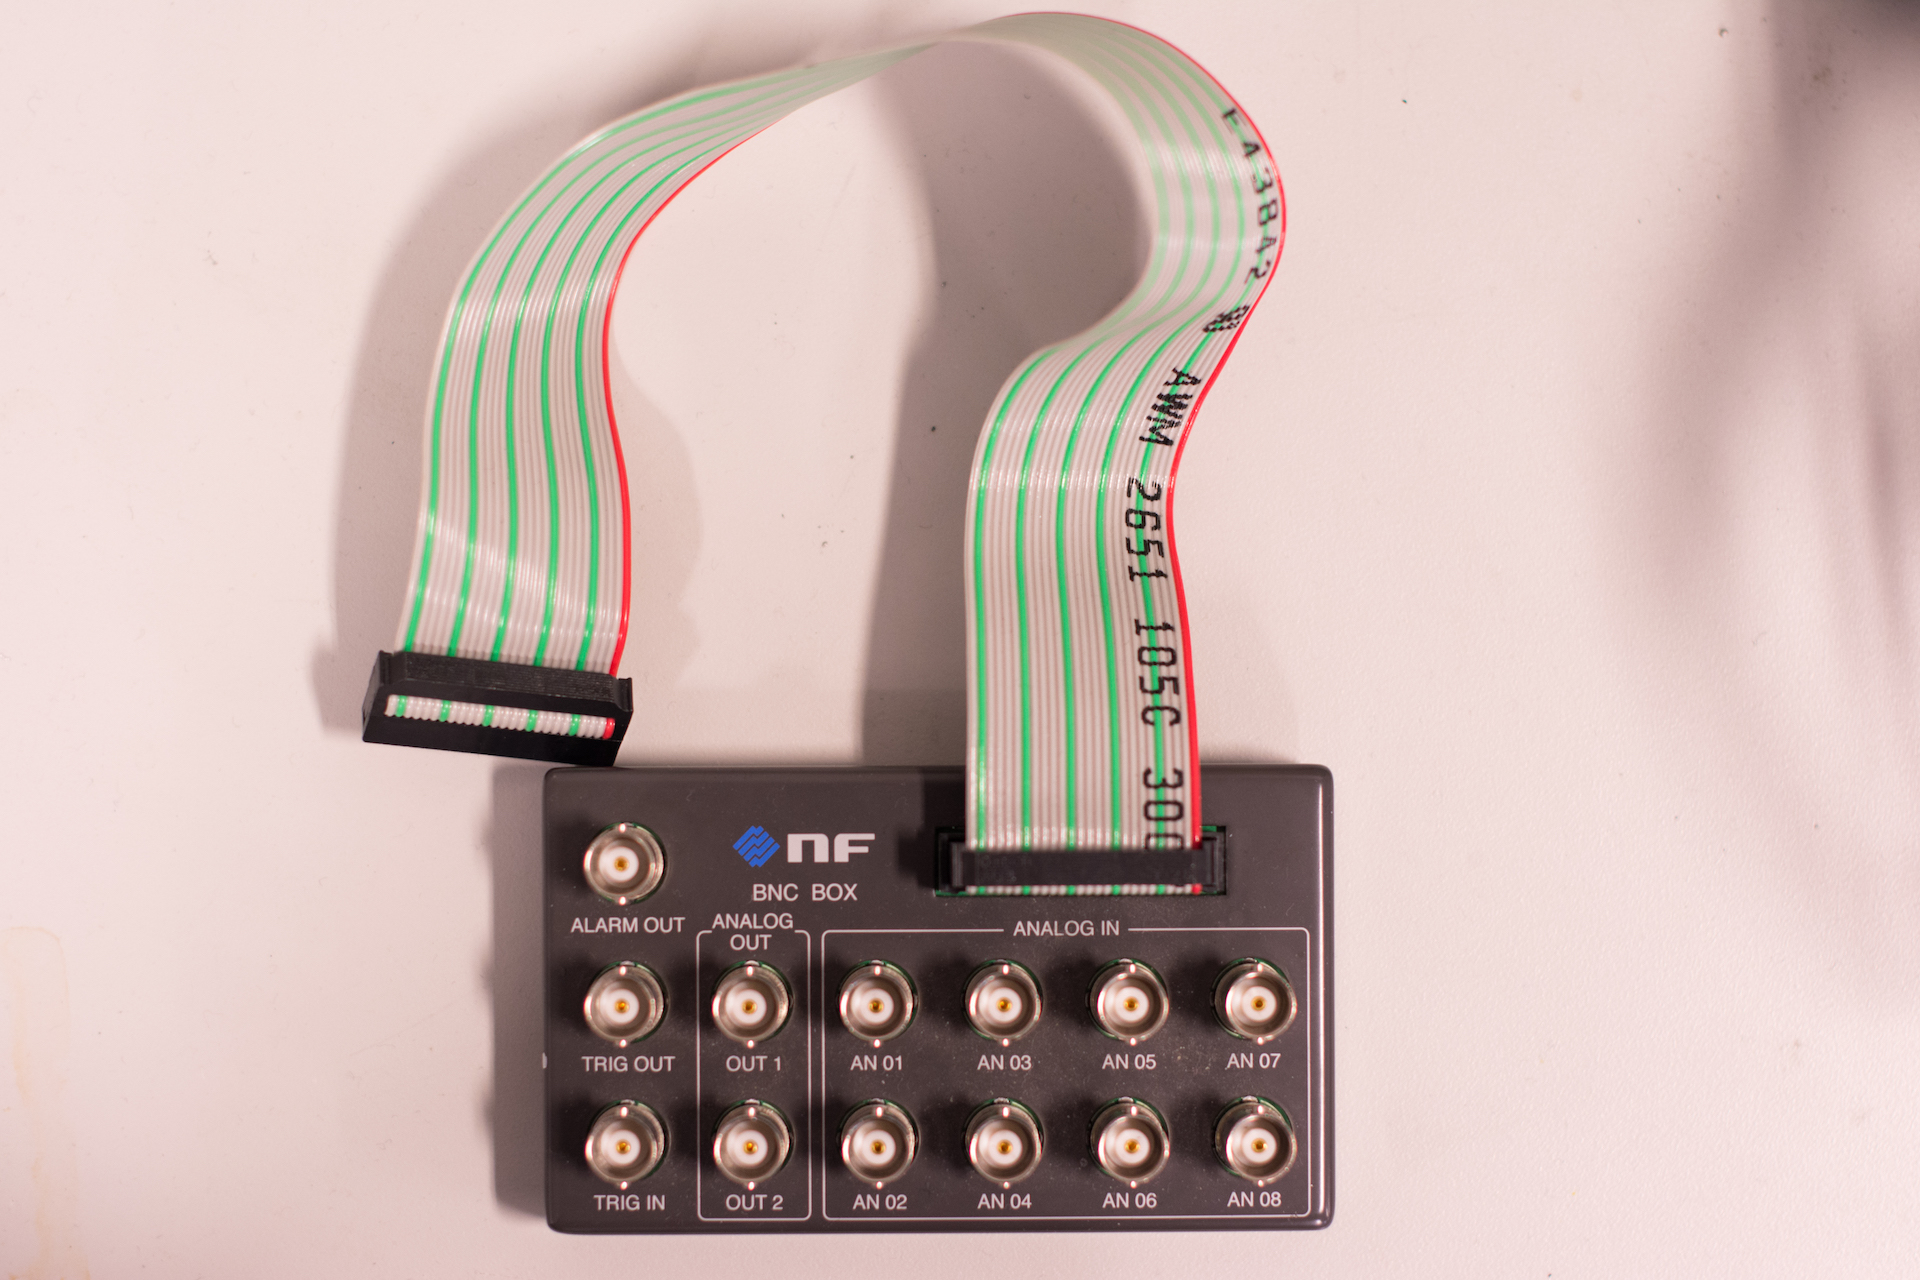
\includegraphics[width=0.6\linewidth]{./figure/bncbox.jpg}
            \end{figure}
        \subsection*{アイソレーショントランス}
        \subsection*{8ch BNCケーブル}
            \begin{figure}[H]
                \centering
                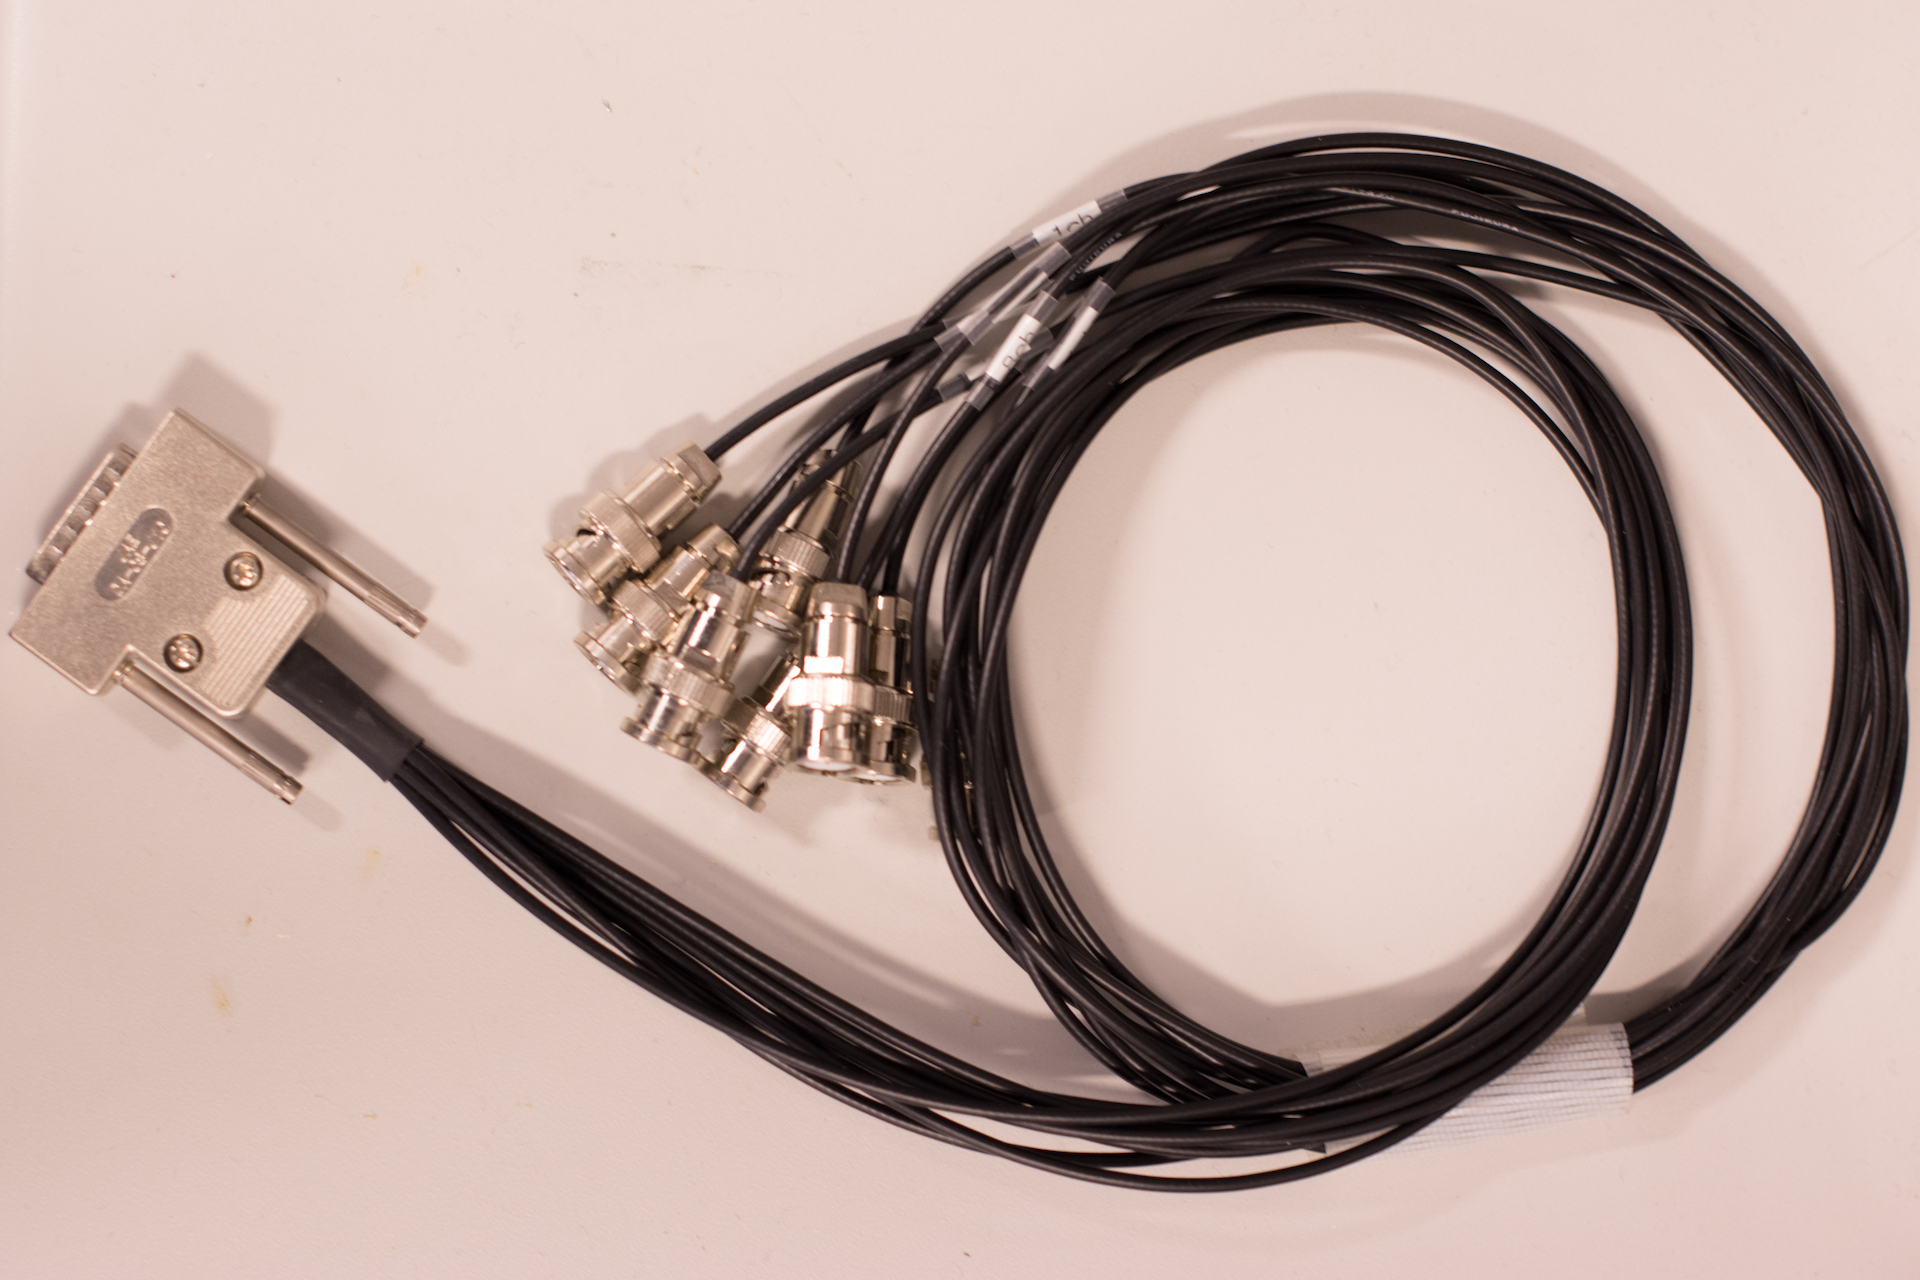
\includegraphics[width=0.6\linewidth]{./figure/bnc-8ch.jpg}
            \end{figure}
        \subsection*{電極}
        \subsection*{ペースト}
            \begin{figure}[H]
                \centering
                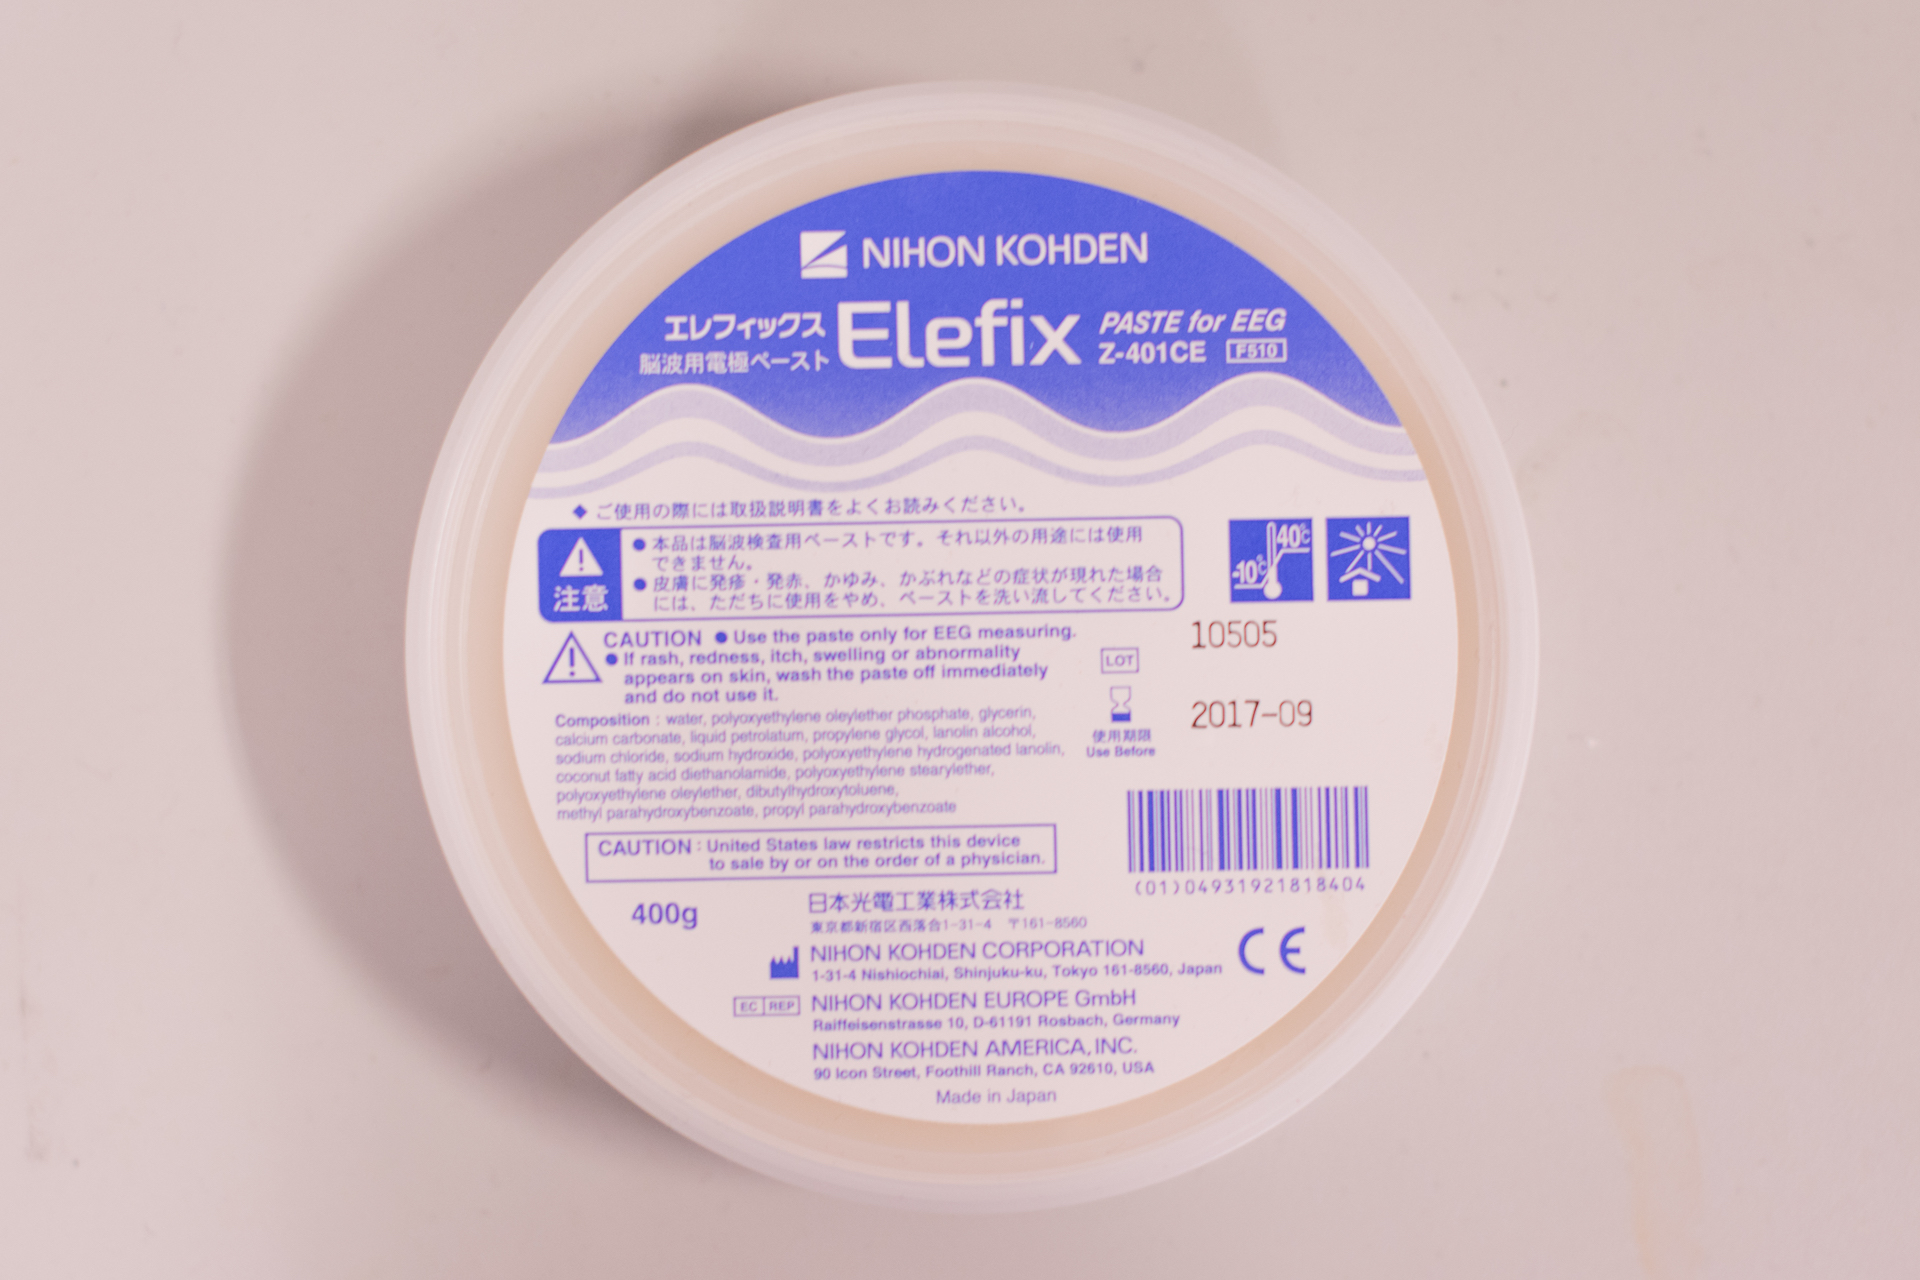
\includegraphics[width=0.6\linewidth]{./figure/elefix.jpg}
            \end{figure}
            冷蔵庫保管.使用期限に注意.
        \subsection*{スキンピュア}
            \begin{figure}[H]
                \centering
                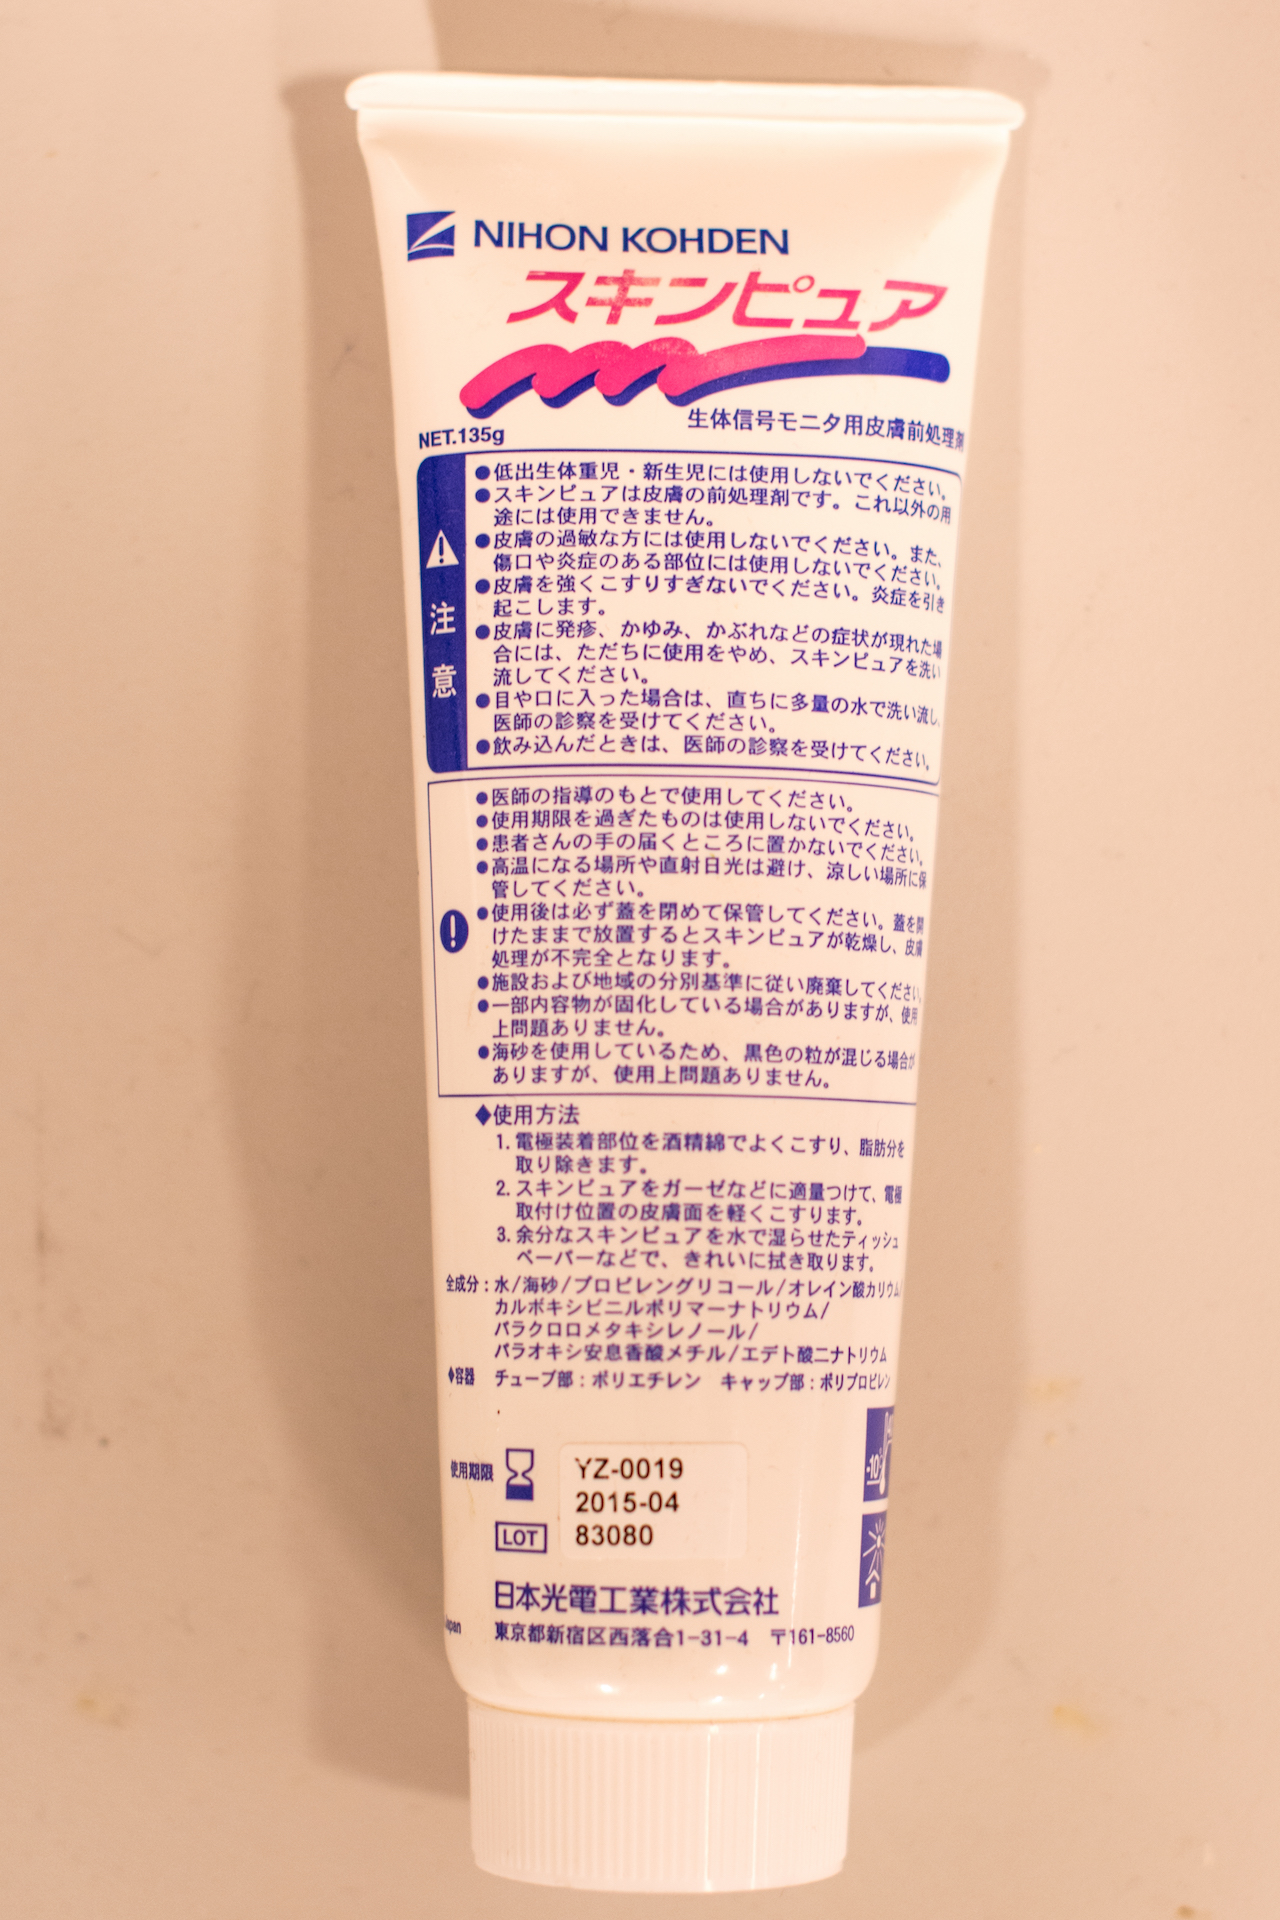
\includegraphics[width=0.5\linewidth]{./figure/skinpure.jpg}
            \end{figure}
        \subsection*{食塩}
        \subsection*{ミルトン}
            どらっぐぱぱす\footnote{豊洲フォレシアにある.}で売ってる.
        \subsection*{綿棒}
            ペーストをすくったりスキンピュアを塗るのに使う.
        \subsection*{ティシュー}
            いろいろ拭き取るのに使う.
        \subsection*{アルコールティシュー\footnote{ノンアルコールでない\textgt{ウェットティシュー}.アロエエキスとかは気にしなくて良い気がする.}}
            いろいろ拭き取るのに使う.
        \subsection*{サージカルテープ}
            電極を固定するのに使う.
        \subsection*{インピーダンス計}
            \begin{figure}[H]
                \centering
                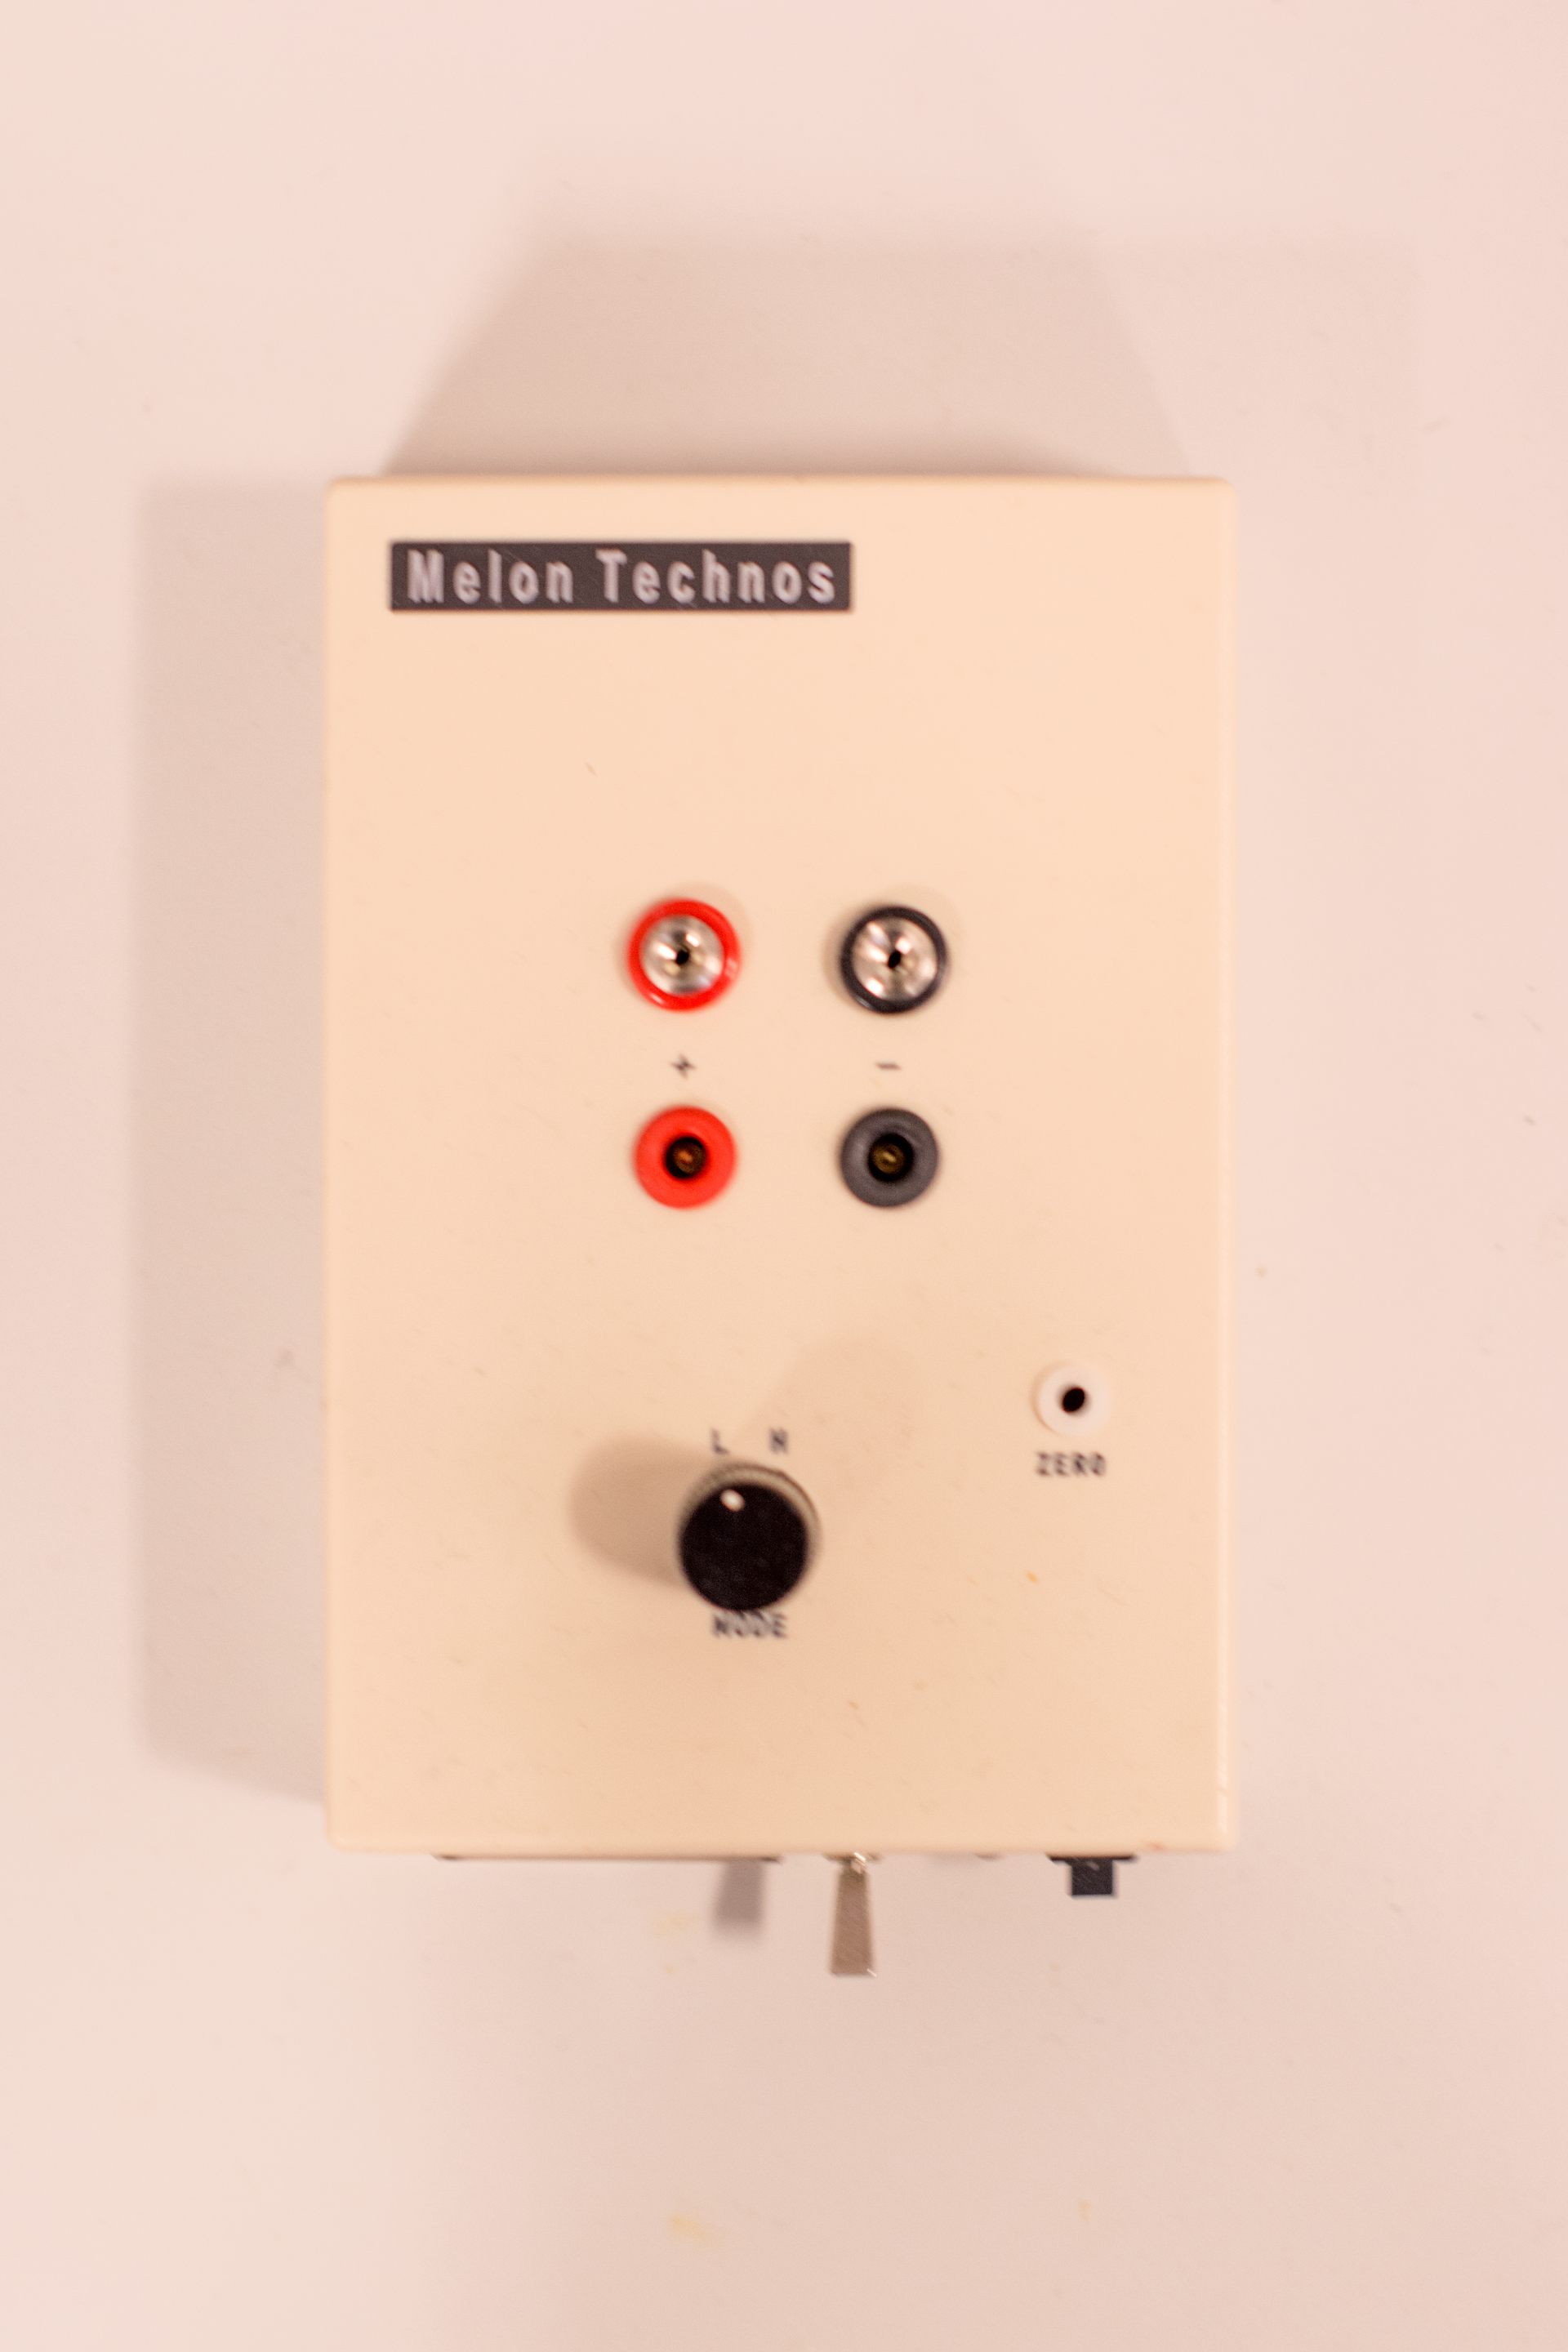
\includegraphics[width=0.5\linewidth]{./figure/impedance.jpg}
            \end{figure}
            9V積層電池で動作する.

    \section{測定の前に}
    \label{sec:section label}
    \begin{itemize}
        \item \textbf{\gtfamily 生体アンプのバッテリは充電してください}.赤いランプが点いている間は充電中です.
        \item \textbf{\gtfamily 電極を生理食塩水に浸してください}.生理食塩水は,水1リットルに対して塩9グラムを溶かします\footnote{水は沸騰させたほうが良いという話もあるが,たいてい水道水をそのまま使う.}.
    \end{itemize}

    \section{測定システム構成}
    \label{sec:測定システム構成}

        システムの概略図は図のとおりです.

        \begin{figure}[H]
            \centering
            \begin{tikzpicture}[every node/.style={draw, rectangle, minimum height=1cm, text centered, text width=2.5cm, font=\sffamily\small, distance=0.5cm}]
                \node(Subj) at (0, 0) {被験者};
                \node[below =0.5cm of Subj] (Amp) {生体アンプ};
                \node[below =0.5cm of Amp] (BNC) {BNCボックス};
                \node[below =0.5cm of BNC] (NF) {データレコーダ};
                \node[left =0.5cm of NF] (Arduino) {Arduinoなど};
                \node[below =0.5cm of NF] (trans) {トランス};
                \node[below =0.5cm of trans] (power) {商用電源};
                \foreach \u / \v in {Subj/Amp, Amp/BNC, BNC/NF, NF/trans, Arduino/NF, trans/power}
                    \draw (\u) -- (\v);
                \path (Arduino) ++(0, -1.5) coordinate(p);
                \draw (Arduino) -- (p) -- (trans);
            \end{tikzpicture}
            \caption{測定システムの構成図}
            \label{測定システム}
        \end{figure}

        データレコーダに接続される「\textsf{Arduinoなど}」は省略することができる.接続方法は第~\ref{sec:Arduinoをデータレコーダに接続する}章に説明する.

    \chapter{一般的な測定}
    \label{chap:一般的な測定}

    ここでは,生体信号のみ計測する場合の方法\footnote{脳波に限らず生体信号全般において共通の方法.}を示す.

        \section{機器を接続する}
        \label{sec:機器を接続する}

            \begin{enumerate}
                \item アイソレーショントランスを適当なコンセントから引っ張ってくる.タコ足配線はしない.
                \item データレコーダのACアダプタを,アイソレーショントランスに接続する.さらに,BNCボックスをデータレコーダのアナログ端子に接続する.
                \begin{figure}[H]
                    \centering
                    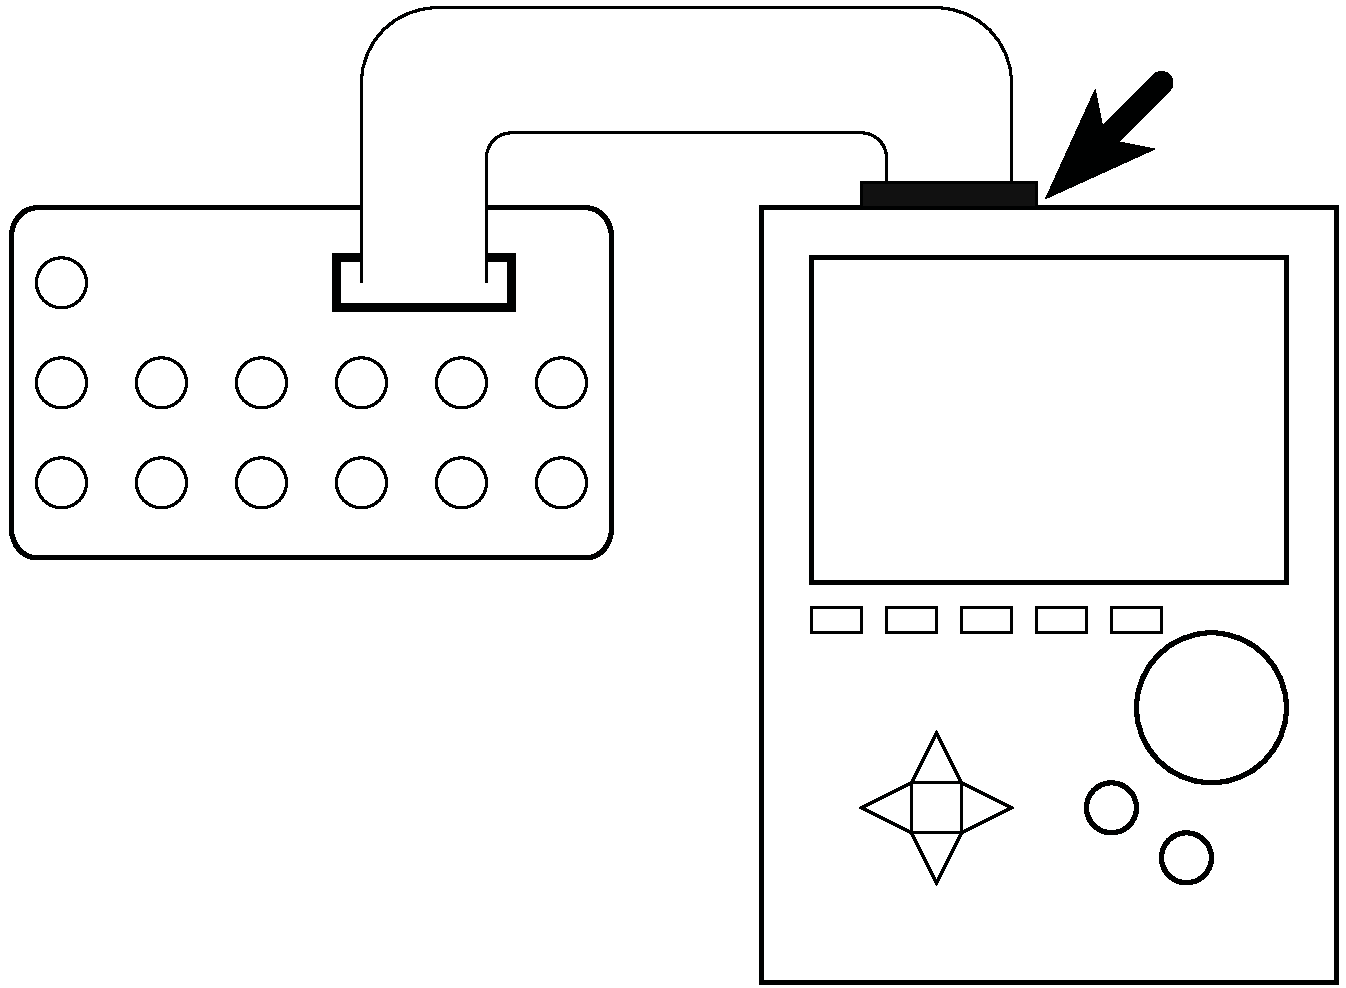
\includegraphics[width=\linewidth]{./figure/bnctonf.pdf}
                    \caption{BNCボックスの接続場所}
                \end{figure}
                \item 8ch BNCケーブルのBNC端子をBNCボックスに接続する.ケーブルごとに対応するチャンネルがあることに注意.さらに,もう一方のコネクタを生体アンプの裏側の端子に接続する.
                \item 生体アンプのバッテリを生体アンプに接続する.
                \item データレコーダの電源を入れる.
                \item 生体アンプの電源を入れる.
            \end{enumerate}

        \section{機器の設定}
        \label{sec:機器の設定}

            \subsection{データレコーダ}
            \label{sub:データレコーダ}

            データレコーダでは,記録パラメータにおいて
            \begin{itemize}
                \item サンプリング周波数
                \item 記録チャンネル数(アナログ8ch,デジタル8chまで同時記録可能)
            \end{itemize}
            を設定する.設定方法は取扱説明書を参照する.

            記録パラメータを設定し終えたらオシロスコープに移り,波形を確認する.
            生体アンプの電源が入っており,電極が刺さっているときはアナログ信号の変化が確認できる.

            \subsection{生体アンプ}
            \label{sub:生体アンプ}

            生体アンプでは,記録パラメータにおいて
            \begin{itemize}
                \item 増幅率
                \item ローパスフィルタのカットオフ周波数
                \item AC増幅の時定数,またはDC増幅かどうか
                \item COM端子を使うかどうか
            \end{itemize}
            をチャンネルごとに設定できる.
            計測したい生体信号ごとの設定方法は取扱説明書を参照する\footnote{たいていの場合はデータレコーダのオシロスコープを確認しながらパラメータを調整する.}.

        \section{電極の確認}
        \label{sec:電極の確認}

            生理食塩水に浸した電極のうち,使用する電極の端子を生体アンプに接続する.
            電極を生理食塩水から出し入れして,データレコーダのオシロスコープで波形を確認する.すべての電極の波形が動いていれば電極・アンプは正常に動作している.

        \section{電極を貼り付ける}
        \label{sec:電極を貼り付ける}

            電極を貼る前に,電極を貼る部位に対して綿棒とスキンピュア,アルコールティシューを使い,皮膚の前処理を行なう.ある程度拭き取ったら,電極を生理食塩水から取り出し,ペーストを綿棒で塗り,貼り付ける.貼り付けた電極はサージカルテープで固定するとよい.

        \section{インピーダンスの確認}
        \label{sec:インピーダンスの確認}

            すべての電極を貼り付けたら,基準電極を-側,記録する電極を+側としてインピーダンス計に挿す.インピーダンス計の電源を入れ,レバーを押すとインピーダンスが測定される.レバーを押してすぐの値を確認し,10k$\Omega$以下であることを確認する.10k$\Omega$を超えた場合は,電極の貼り付け具合を確認するか,電極を取り替えて再度行なう.

            この操作をすべての記録する電極に対して行なう\footnote{この操作は省略する場合もある.}.

        \section{データレコーダの確認}
        \label{sec:データレコーダの確認}

            データレコーダのオシロスコープを確認する.波形が変化しない場合は
            \begin{itemize}
                \item 電極がすべて貼り付けられているか
                \item 生体アンプの増幅率は適切か
                \item 生体アンプの電源は入っているか
                \item 電極に不具合はないか
                \item データレコーダのチャンネルとアンプのチャンネルの対応
            \end{itemize}
            を確認する.

        \section{測定}
        \label{sec:測定}

            データレコーダの``\textsf{RECORD}''を押すとすぐに記録が開始される.終了するときはもう一度``\textsf{RECORD}''を押すと記録を終了する.

        \section{片付け}
        \label{sec:片付け}

        測定を終了するときは,すべての機器の電源を切り,電極を剥がす.皮膚をアルコールティシューで拭き,電極についたペーストも拭き取る.電極を生体アンプから外し,水道水で洗う.生理食塩水の入った容器も洗う.生体アンプの電源ケーブル,データレコーダの電源ケーブルを外し,適当にまとめる.

        ミルトン容器に水道水1リットルを用意し,ミルトンを適量混ぜる.電極の先を浸し,ケーブルは電極置きに吊り下げる.ケーブルを浸しすぎるとボロボロになるので注意する.

        最後に機器,机などの汚れた部分を拭きとって終了.ゴミはかならず捨てる.

        翌日,ミルトンに浸した電極を取り出し,ミルトン容器を洗う\footnote{ミルトンに浸したまま一週間放置はよくあるので忘れないこと.}.

    \chapter{データの抽出}
    \label{chap:データの抽出}

    データレコーダからのデータ抽出には,ソフトウエア``0751''を使用する.もしインストールされていなければ,\texttt{\textbackslash\textbackslash TS-XHL4F7\textbackslash seminar\textbackslash Application\textbackslash データレコーダーEZ7510用\textbackslash setup.exe}からインストールする.
    ライセンスキーは\texttt{readme.txt}の最終行に記載されている.

        \section{ファイルを開く}

        データレコーダをPCにUSB接続する.
        0751を起動して,``ファイル''→``開く''をクリックする.
        次に``ファイル名''→``新しく開く''をクリックする.
        データレコーダの``Data''ディレクトリには日時順に連番でファイルが保存されているので,
        該当するDATファイルを選択する.

        取り出したいデータのチャンネルを選択し,``引当''をクリックすると,右側のテーブルに選択したチャンネルが移動する.
        \begin{figure}[H]
            \centering
            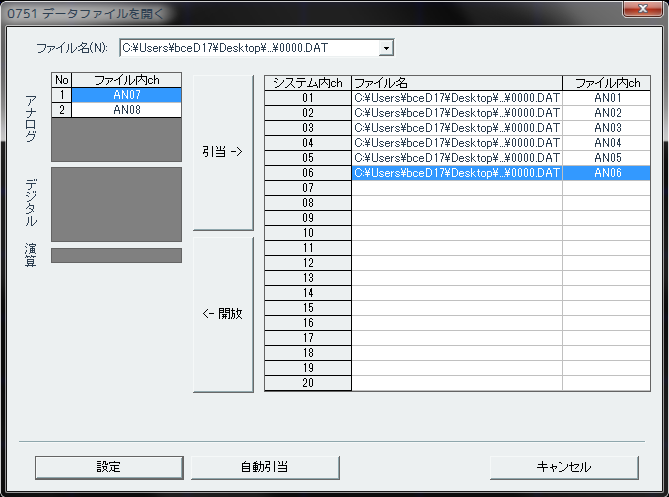
\includegraphics[width=\linewidth]{./figure/0751-open.png}
            \caption{データファイルを開く}
        \end{figure}
        ``設定''をクリックすると,波形が表示される.
        \begin{figure}[H]
            \centering
            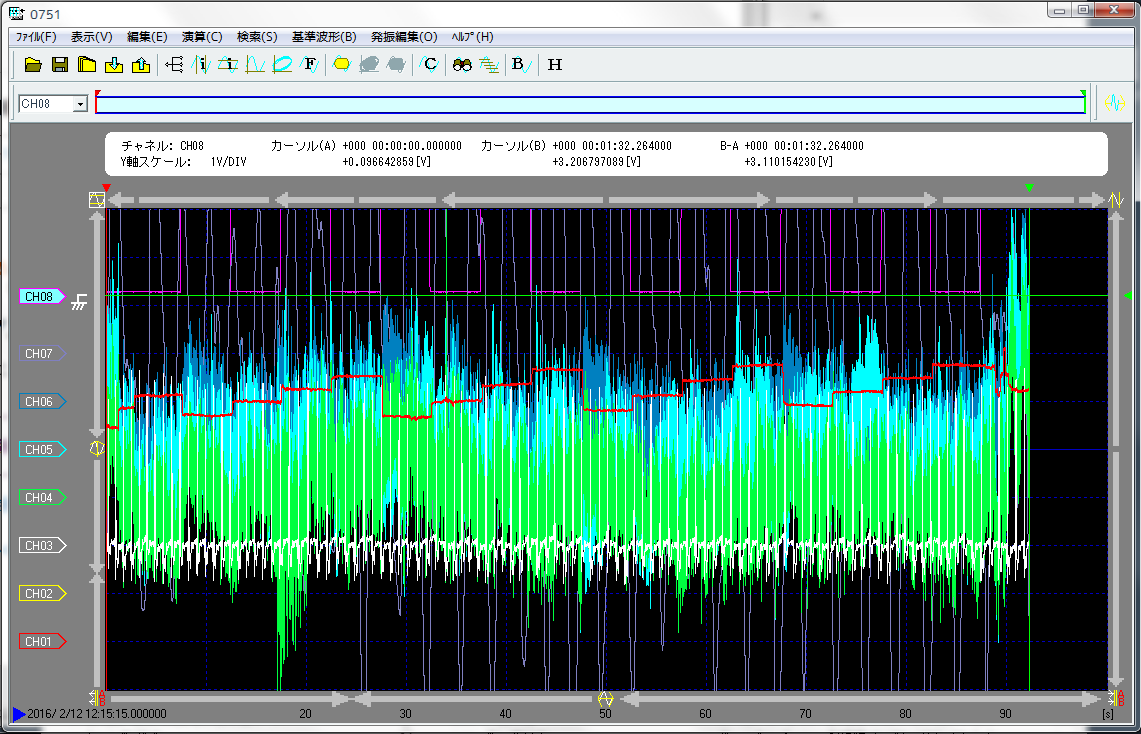
\includegraphics[width=\linewidth]{./figure/0751-wave.png}
            \caption{波形表示画面}
        \end{figure}
        \section{データのエクスポート}

        ``ファイル''→``エクスポート''をクリックする.チャンネルを選択し,保存形式をバイナリにして``実行''をクリックする.

        \begin{figure}[H]
            \centering
            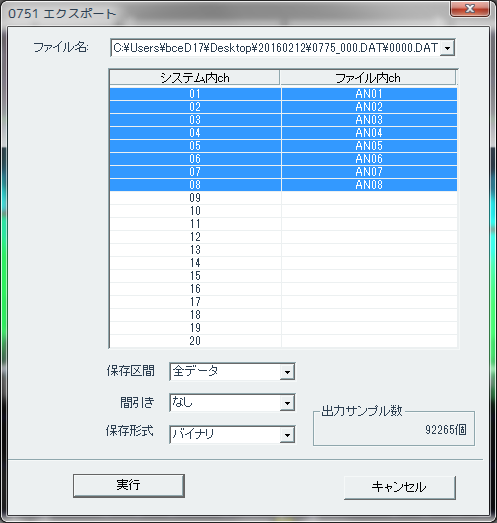
\includegraphics[width=\linewidth]{./figure/0751-export.png}
            \caption{エクスポート画面}
        \end{figure}
        適当なファイル名をつけて保存すると,バイナリファイルが生成される.バイナリファイルの構造については,取扱説明書を参照すること.
    \chapter{補足}
    \label{chap:補足}

        \section{Arduinoをデータレコーダに接続する}
        \label{sec:Arduinoをデータレコーダに接続する}

        ここではArduinoで0,5Vのデジタル出力を行ない,出力をデータレコーダに記録する方法を説明する\footnote{アナログ出力はPWMとして実現されるが,ここでは省略する.}.データレコーダではデジタル入力を同時に8chぶん計測できる.

        データレコーダのデジタル端子とテストクリップがついたケーブルを用いる.カラーとチャンネルは対応づけられている.適当なクリップを回路中に取り付け,もう一方の端子をデータレコーダに接続する.黒いテストクリップは回路中のGNDに取り付ける.

        \begin{figure}[H]
            \centering
            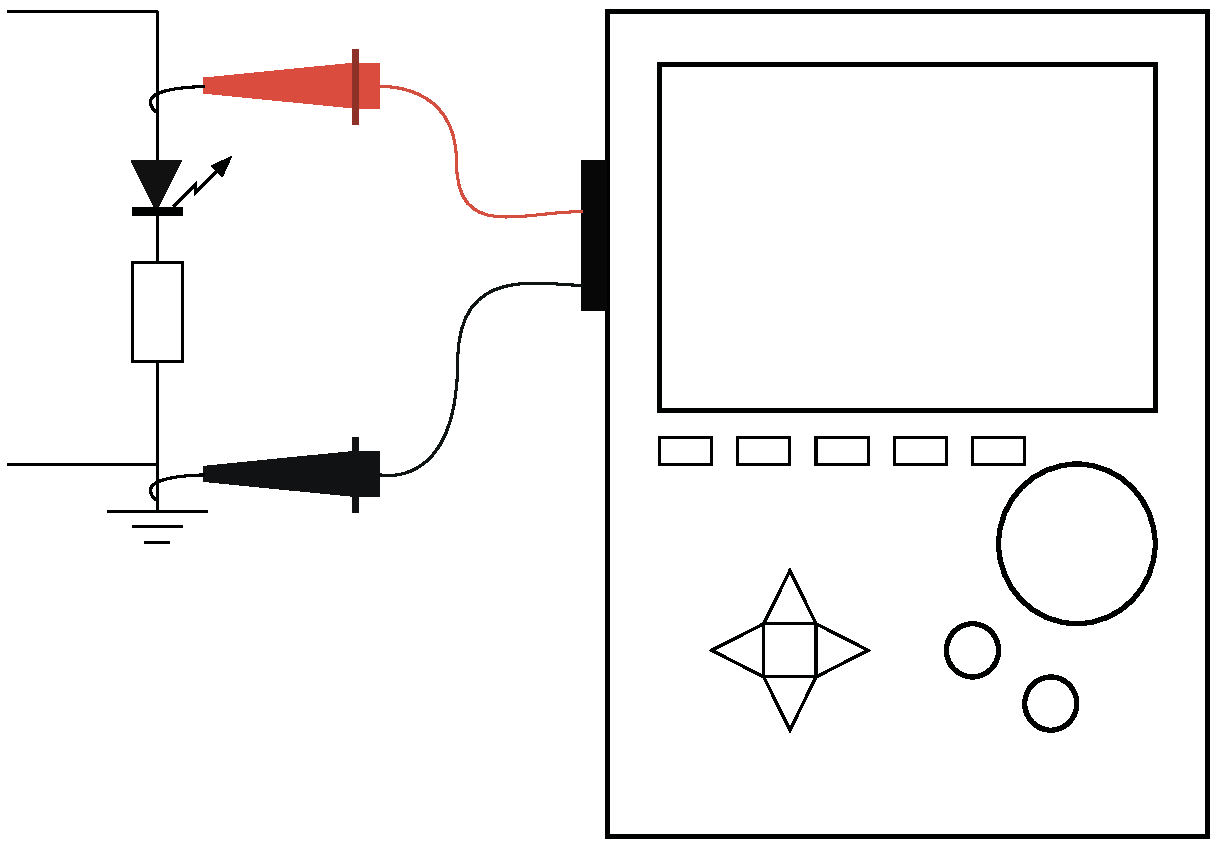
\includegraphics[width=\linewidth]{./figure/digital-testclip.pdf}
            \caption{データレコーダと回路の接続例}
        \end{figure}

        データレコーダでデジタル入力の設定を行ない,オシロスコープを確認する.記録されるデータは0または1の数値となる.

        \section{回路中の電圧をアナログ信号として記録する}
        \label{sec:回路中の電圧をアナログ信号として記録する}

        もし回路中の電圧を0,1の2値ではなく連続的な値として記録したい場合,BNC-ワニ口ケーブルをBNCボックスの任意のチャンネルに接続する.このとき,生体アンプから接続されていたBNCのうち1つ以上はBNC-ワニ口ケーブルに使用されることに注意.

        ワニ口クリップを回路中に接続したら,オシロスコープを確認する.

        \begin{figure}[H]
            \centering
            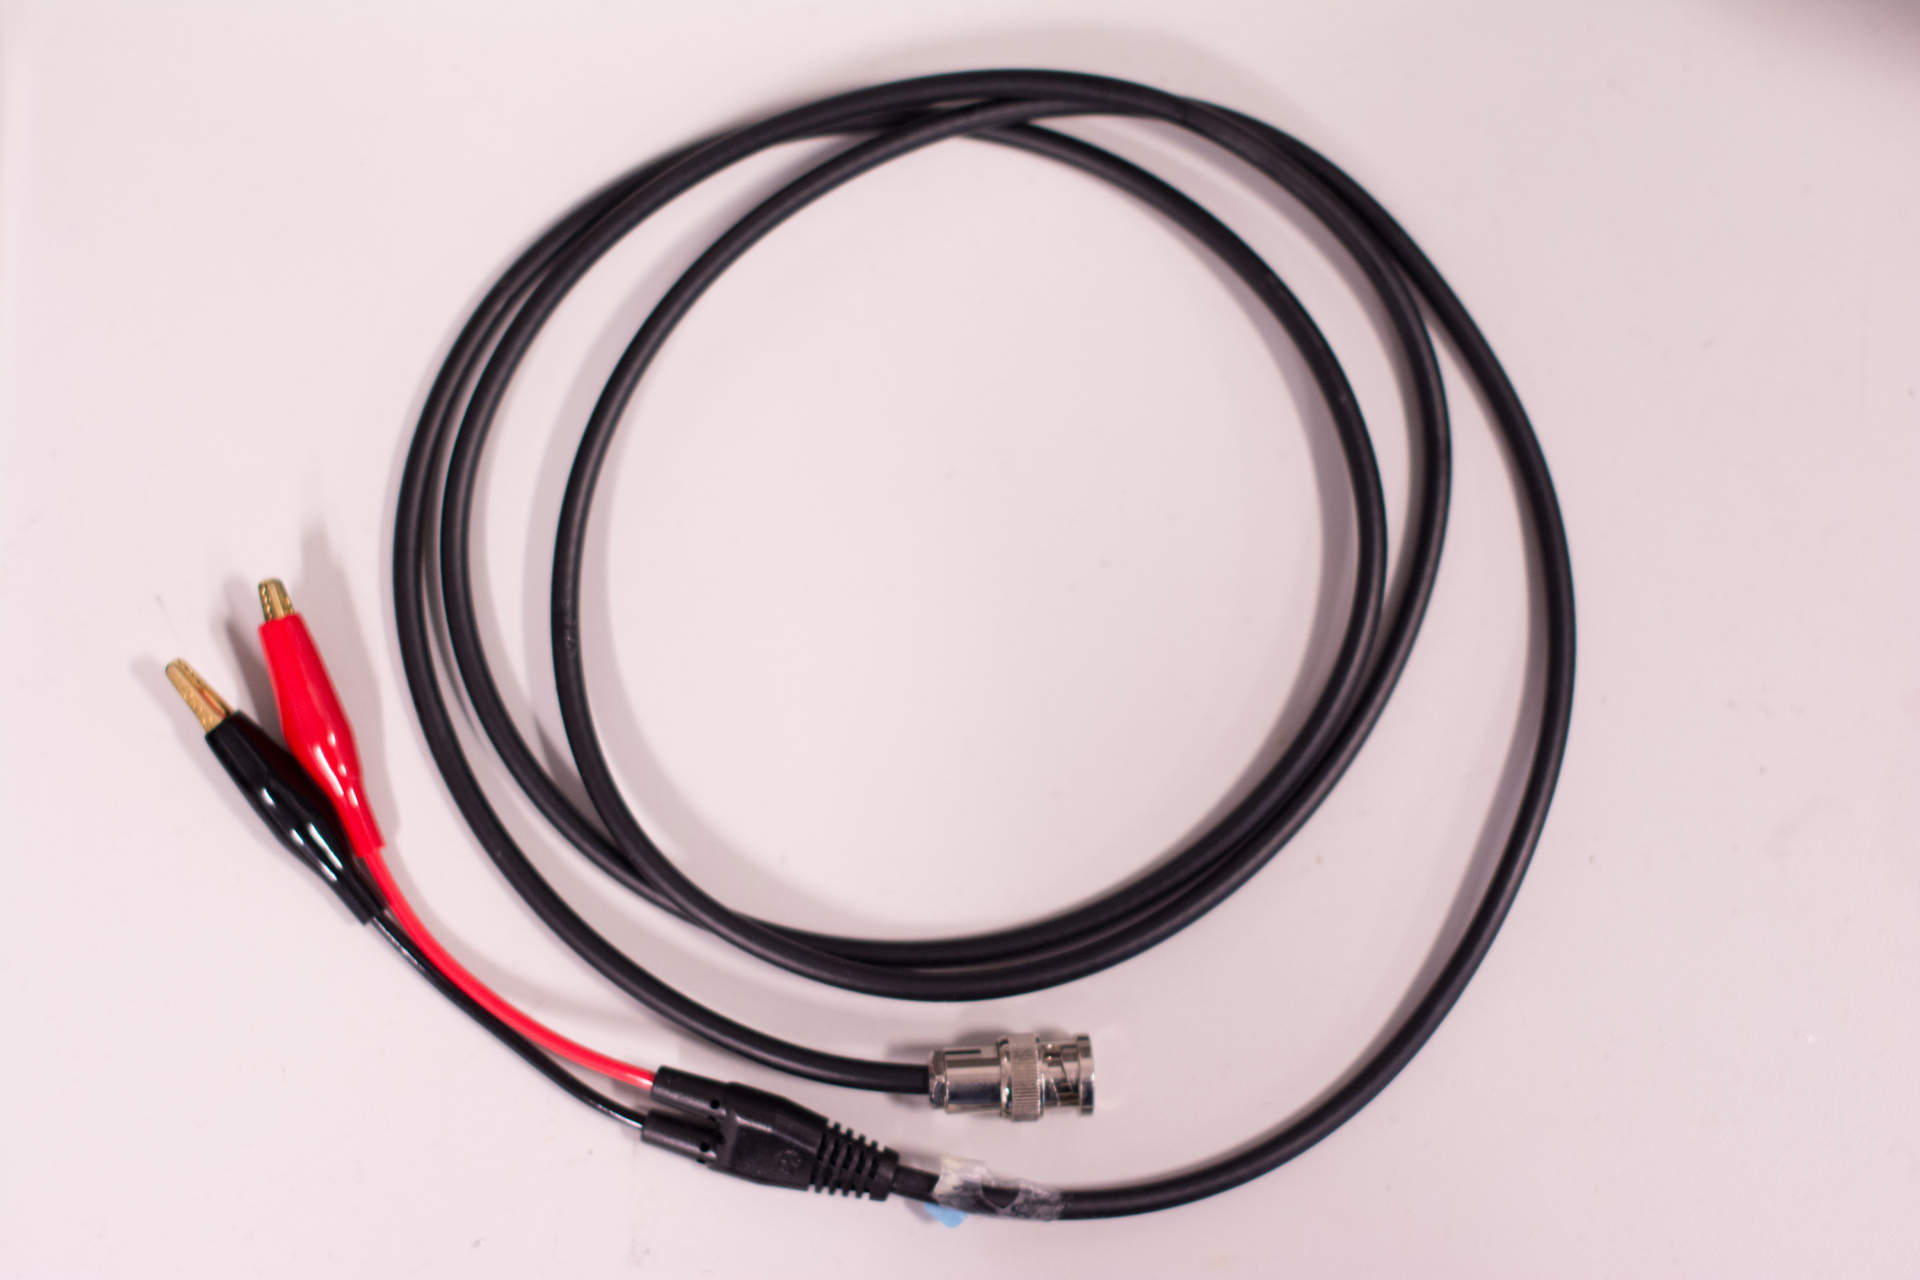
\includegraphics[width=\linewidth]{./figure/bnc-alligator.jpg}
            \caption{BNC-ワニ口ケーブル}
        \end{figure}

        \section{生体計測に関する補足}
        \label{sec:生体計測に関する補足}

        以下の書籍に生体計測に関する情報が載っている.

        \begin{itemize}
            \item ``\textsf{ヒト心身状態の計測技術
- 人に優しい製品開発のための日常計測 -}''(コロナ社):脳波のほか,筋電図,眼電図についての計測方法が詳細に書かれている.目的に合わせて読むとよい.
            \item ``\textsf{標準生理学}''(医学書院):生体信号の発生機序を知りたい場合はこちら.
            \item ``\textsf{脳波の旅への誘い 第2版}''(星和書店)
            \item ``\textsf{バイオメカニズム・ライブラリー 表面筋電図}''(東京電機大学出版局)
        \end{itemize}

        \section{分析ツール}
        \label{sec:分析ツール}

            分析方法は生体信号や目的によってさまざまだが,分析ツールには以下がよく使われる.

            \begin{itemize}
                \item \textsf{MATLAB}:研究室のデファクトスタンダード的なソフトウエア.大規模な配列処理が可能で,公式ドキュメントが豊富.有償・無償問わずさまざまなToolboxがある(EEGLAB, Psychtoolboxはときどき使っていた).
                \item \textsf{Python}:オープンソース・ソフトウェアで,ライブラリNumpy, Scipyを用いることで高速な行列計算・信号処理が可能になる.ライブラリが豊富で,アプリケーションとして実装が可能.
                \item \textsf{R}:オープンソース・ソフトウェアで,データ整形や統計処理・可視化を得意とする.動作はそれほど高速ではない.
                \item \textsf{Excel}:アドイン``分析ツール''を使うことで,検定や回帰分析を行なうことができる.データの数が膨大だと動作が不安定になるので注意.
            \end{itemize}

    \clearpage
    \appendix
    \chapter{生体アンプ取扱説明書}
    \includepdf[pages=-]{./figure/amp-manual.pdf}

\end{document}
